\documentclass{article}
\usepackage[dvipdfm]{graphicx}
\usepackage[dvipdfm]{color}
\usepackage[dvipdfm]{hyperref}
\title{\color{blue}Latex Support Test File}
\author{\color{green}Mark A. Wicks}
\begin{document}
\maketitle
\section{Introduction}
This document is primarily intended
to demonstrate the functionality
of some \LaTeX packages that require
driver support for their functionality.
It is quick-and-dirty.
It is not intended to be pretty, and
does not demonstrate good ways to use these packages
(In fact, it demonstrates some bad ways to use these packages).

\section{Driver Files}
This distribution of {\tt dvipdfm} includes
the {\tt .def} files required to support
the \textcolor{green}{color},
\rotatebox{30}{\textcolor{red}{graphics}}, and hyperref \LaTeX\space
packages.  Once these .def files
are installed where these packages
can find them.  You also may need
to modify {\tt color.sty}, {\tt graphics.sty},
and {\tt hyperref.sty} so that they
recognize {\tt dvipdfm} as a driver.
Once these {\tt .def} files are installed,
you should be able to use {\tt dvipdfm}
with \LaTeX for many applications.

After running \LaTeX on this
document, {\tt hyperref}
should produce a hyperlinked
document, complete with an outline.

\newpage
\section{Graphics Support}
Currently, JPEG and PDF image
inclusion are supported.

\subsection{JPEG Image Inclusion}
Figure~\ref{fig:author}
shows a photograph of the author
that was obtained from a JPEG file.
A small file with the extension of {\tt .bb}
supplies the bounding box to the \LaTeX\space
Graphics package.  For PDF and JPEG files,
this bounding box can easily be created by running
the {\tt ebb} utility included with this
distribution of {\tt dvipdfm}.

\begin{figure}
  \begin{center}
    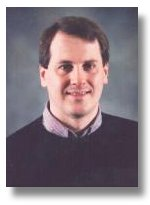
\includegraphics{mwicks.jpeg}
  \end{center}

  \caption{A photograph of the author.}
  \label{fig:author}
\end{figure}

\subsection{PDF Image Inclusion}
Figure~\ref{fig:circuit} shows
an electronics circuit,
drawn with XFig, distilled,
and then included as PDF file.
\begin{figure}
  \begin{center}
     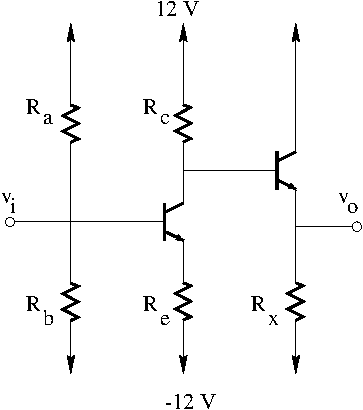
\includegraphics{transistor.pdf}
  \end{center}

  \caption{A simple two-stage transistor circuit.}
  \label{fig:circuit}
\end{figure}

\begin{figure}
  \begin{center}
     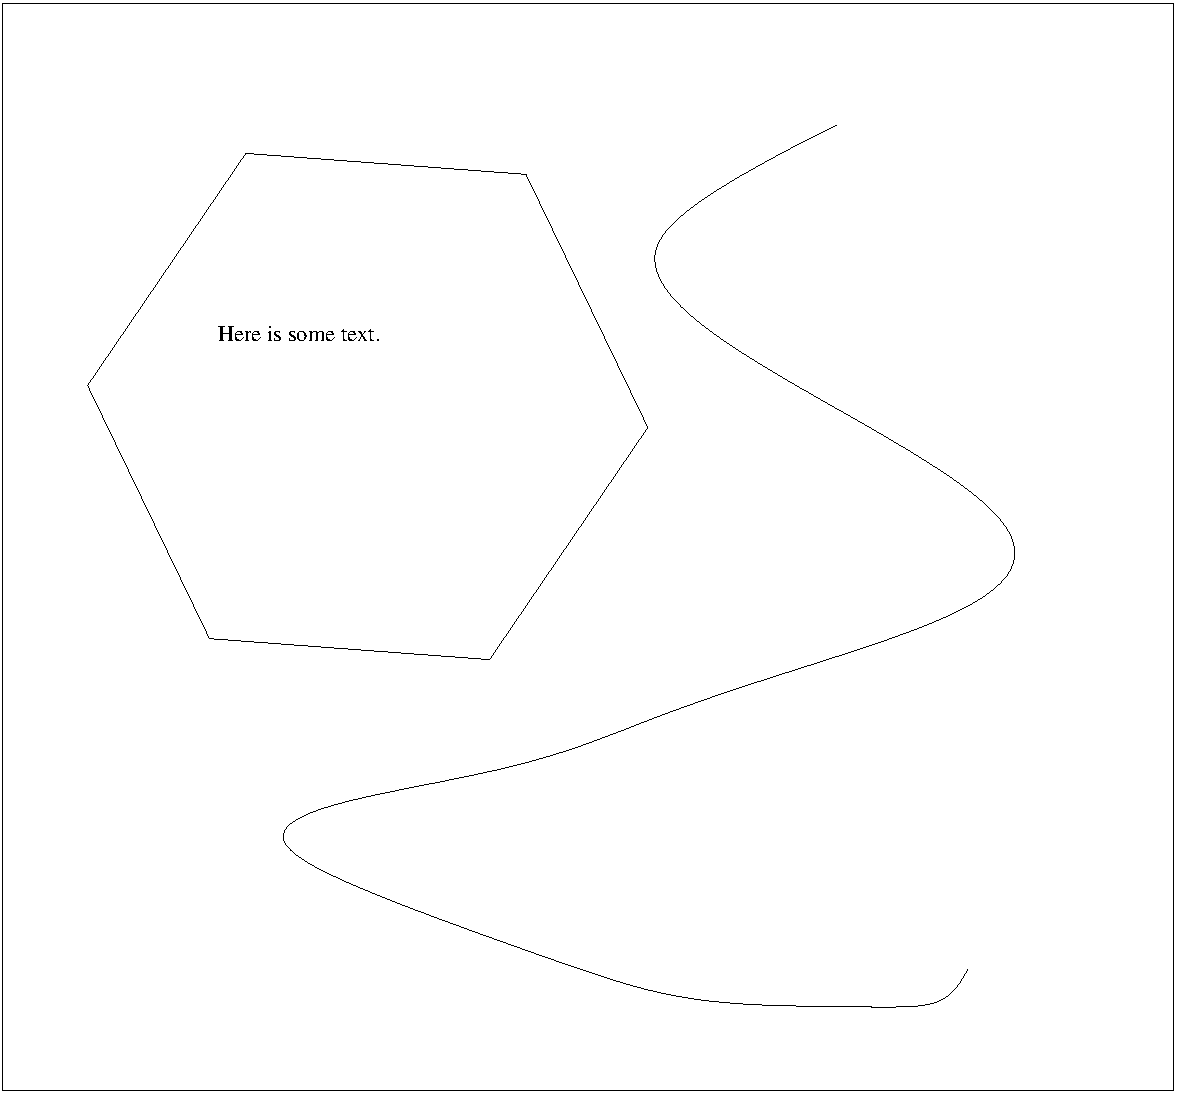
\includegraphics[width=3.0in]{something.pdf}
  \end{center}

  \caption{A second included figure}
  \label{fig:something}
\end{figure}

\end{document}
